\documentclass[slidestop]{beamer}
\usepackage{beamerthemesplit}
\usepackage{graphics}
\usepackage{pstricks}

\title{Simple-V RISC-V Extension for Vectorisation and SIMD}
\author{Luke Kenneth Casson Leighton}


\begin{document}

\frame{
   \begin{center}
    \huge{Simple-V RISC-V Extension for Vectors and SIMD}\\
    \vspace{32pt}
    \Large{Flexible Vectorisation}\\
    \Large{(aka not so Simple-V?)}\\
    \vspace{24pt}
    \Large{[proposed for] Chennai 9th RISC-V Workshop}\\
    \vspace{24pt}
    \large{\today}
  \end{center}
}


\frame{\frametitle{Credits and Acknowledgements}

 \begin{itemize}
   \item The Designers of RISC-V\vspace{15pt}
   \item The RVV Working Group and contributors\vspace{15pt}
   \item Allen Baum, Jacob Bachmeyer, Xan Phung, Chuanhua Chang,\\
	     Guy Lemurieux, Jonathan Neuschafer, Roger Brussee,
	     and others\vspace{15pt}
   \item ISA-Dev Group Members\vspace{10pt}
  \end{itemize}
}


\frame{\frametitle{Quick refresher on SIMD}

 \begin{itemize}
   \item SIMD very easy to implement (and very seductive)\vspace{10pt}
   \item Parallelism is in the ALU\vspace{10pt}
   \item Zero-to-Negligeable impact for rest of core\vspace{10pt}
  \end{itemize}
  Where SIMD Goes Wrong:\vspace{10pt}
   \begin{itemize}
   \item See "SIMD instructions considered harmful"
   https://www.sigarch.org/simd-instructions-considered-harmful
   \item Corner-cases alone are extremely complex.\\
	     Hardware is easy, but software is hell.
   \item O($N^{6}$) ISA opcode proliferation!\\
	     opcode, elwidth, veclen, src1-src2-dest hi/lo
  \end{itemize}
}

\frame{\frametitle{Quick refresher on RVV}

 \begin{itemize}
   \item Extremely powerful (extensible to 256 registers)\vspace{10pt}
   \item Supports polymorphism, several datatypes (inc. FP16)\vspace{10pt}
   \item Requires a separate Register File (32 w/ext to 256)\vspace{10pt}
   \item Implemented as a separate pipeline (no impact on scalar)\vspace{10pt}
  \end{itemize}
  However...\vspace{10pt}
   \begin{itemize}
   \item 98 percent opcode duplication with rest of RV (CLIP)
   \item Extending RVV requires customisation not just of h/w:\\
	     gcc and s/w also need customisation (and maintenance)
  \end{itemize}
}


\frame{\frametitle{The Simon Sinek lowdown (Why, How, What)}

 \begin{itemize}
   \item Why?
         Implementors need flexibility in vectorisation to optimise for
         area or performance depending on the scope:
	     embedded DSP, Mobile GPU's, Server CPU's and more.\vspace{4pt}\\
		 Compilers also need flexibility in vectorisation to optimise for cost 
		 of pipeline setup, amount of state to context switch
		 and software portability\vspace{4pt}
   \item How?
	     By implicitly marking INT/FP regs as "Vectorised",\\
	     SV expresses how existing instructions should act 
	     on [contiguous] blocks of registers, in parallel.\vspace{4pt}
   \item What?
		 Simple-V is an "API" that implicitly extends
		 existing (scalar) instructions with explicit parallelisation. 
  \end{itemize}
}


\frame{\frametitle{What's the value of SV? Why adopt it even in non-V?}

 \begin{itemize}
   \item memcpy becomes much smaller (higher bang-per-buck)\vspace{10pt}
   \item context-switch (LOAD/STORE multiple): 1-2 instructions\vspace{10pt}
   \item Compressed instrs further reduces I-cache (etc.)\vspace{10pt}
   \item greatly-reduced I-cache load (and less reads)\vspace{10pt}
  \end{itemize}
  Note:\vspace{10pt}
   \begin{itemize}
   \item It's not just about Vectors: it's about instruction effectiveness
   \item Anything implementor is not interested in HW-optimising,\\
	     let it fall through to exceptions (implement as a trap).
  \end{itemize}
}


\frame{\frametitle{How does Simple-V relate to RVV?}

 \begin{itemize}
   \item RVV very heavy-duty (excellent for supercomputing)\vspace{10pt}
   \item Simple-V abstracts parallelism (based on best of RVV)\vspace{10pt}
   \item Graded levels: hardware, hybrid or traps (fit impl. need)\vspace{10pt}
   \item Even Compressed instructions become vectorised\vspace{10pt}
  \end{itemize}
  What Simple-V is not:\vspace{10pt}
   \begin{itemize}
   \item A full supercomputer-level Vector Proposal
   \item A replacement for RVV (SV is designed to be over-ridden\\
	     by - or augmented to become, or just be replaced by  - RVV)
  \end{itemize}
}


\frame{\frametitle{How is Parallelism abstracted in Simple-V?}

 \begin{itemize}
   \item Register "typing" turns any op into an implicit Vector op\vspace{10pt}
   \item Primarily at the Instruction issue phase (except SIMD)\\
         Note: it's ok to pass predication through to ALU (like SIMD)
   \item Standard (and future, and custom) opcodes now parallel\vspace{10pt}
  \end{itemize}
  Notes:\vspace{6pt}
   \begin{itemize}
   \item All LOAD/STORE (inc. Compressed, Int/FP versions)
   \item All ALU ops (soft / hybrid / full HW, on per-op basis)
   \item All branches become predication targets (C.FNE added)
   \item C.MV of particular interest (s/v, v/v, v/s)
  \end{itemize}
}


\frame{\frametitle{Implementation Options}

 \begin{itemize}
   \item Absolute minimum: Exceptions (if CSRs indicate "V", trap)
   \item Hardware loop, single-instruction issue\\
		 (Do / Don't send through predication to ALU)
   \item Hardware loop, parallel (multi-instruction) issue\\
   		 (Do / Don't send through predication to ALU)
   \item Hardware loop, full parallel ALU (not recommended)
  \end{itemize}
  Notes:\vspace{6pt}
  \begin{itemize}
   \item 4 (or more?) options above may be deployed on per-op basis
   \item SIMD always sends predication bits through to ALU
   \item Minimum MVL MUST be sufficient to cover regfile LD/ST
   \item Instr. FIFO may repeatedly split off N scalar ops at a time
  \end{itemize}
}
% Instr. FIFO may need its own slide.  Basically, the vectorised op
% gets pushed into the FIFO, where it is then "processed".  Processing
% will remove the first set of ops from its vector numbering (taking
% predication into account) and shoving them **BACK** into the FIFO,
% but MODIFYING the remaining "vectorised" op, subtracting the now
% scalar ops from it.

\frame{\frametitle{How are SIMD Instructions Vectorised?}

 \begin{itemize}
   \item SIMD ALU(s) primarily unchanged\vspace{10pt}
   \item Predication is added to each SIMD element (NO ZEROING!)\vspace{10pt}
   \item End of Vector enables predication (NO ZEROING!)\vspace{10pt}
  \end{itemize}
  Considerations:\vspace{10pt}
   \begin{itemize}
   \item Many SIMD ALUs possible (parallel execution)\vspace{10pt}
   \item Very long SIMD ALUs could waste die area (short vectors)\vspace{10pt}
   \item Implementor free to choose (API remains the same)\vspace{10pt}
  \end{itemize}
}
% With multiple SIMD ALUs at for example 32-bit wide they can be used 
% to either issue 64-bit or 128-bit or 256-bit wide SIMD operations
% or they can be used to cover several operations on totally different
% vectors / registers.

\frame{\frametitle{What's the deal / juice / score?}

 \begin{itemize}
   \item Standard Register File(s) overloaded with CSR "vector span"\\
	     (see pseudocode slides for examples)
   \item Element width and type concepts remain same as RVV\\
	     (CSRs are used to "interpret" elements in registers)
   \item CSRs are key-value tables (overlaps allowed)\vspace{10pt}
  \end{itemize}
  Key differences from RVV:\vspace{10pt}
   \begin{itemize}
   \item Predication in INT regs as a BIT field (max VL=XLEN)
   \item Minimum VL must be Num Regs - 1 (all regs single LD/ST)
   \item SV may condense sparse Vecs: RVV lets ALU do predication
   \item NO ZEROING: non-predicated elements are skipped
  \end{itemize}
}


\begin{frame}[fragile]
\frametitle{ADD pseudocode (or trap, or actual hardware loop)}

\begin{semiverbatim}
function op_add(rd, rs1, rs2, predr) # add not VADD!
  int i, id=0, irs1=0, irs2=0;
  for (i=0; i < MIN(VL, vectorlen[rd]); i++)
    if (ireg[predr] & 1<<i) # predication uses intregs
       ireg[rd+id] <= ireg[rs1+irs1] + ireg[rs2+irs2];
    if (reg_is_vectorised[rd]) \{ id += 1; \}
    if (reg_is_vectorised[rs1]) \{ irs1 += 1; \}
    if (reg_is_vectorised[rs2]) \{ irs2 += 1; \}
\end{semiverbatim}

  \begin{itemize}
   \item SIMD slightly more complex (case above is elwidth = default)
   \item Scalar-scalar and scalar-vector and vector-vector now all in one
   \item OoO may choose to push ADDs into instr. queue (v. busy!)
  \end{itemize}
\end{frame}

% yes it really *is* ADD not VADD.  that's the entire point of
% this proposal, that *standard* operations are overloaded to
% become vectorised-on-demand


\begin{frame}[fragile]
\frametitle{Predication-Branch (or trap, or actual hardware loop)}

\begin{semiverbatim}
s1 = reg_is_vectorised(src1);
s2 = reg_is_vectorised(src2);
if (!s2 && !s1) goto branch;
for (int i = 0; i < VL; ++i)
   preg[rs3] |= 1 << cmp(s1 ? reg[src1+i] : reg[src1],
                         s2 ? reg[src2+i] : reg[src2]);
\end{semiverbatim}

  \begin{itemize}
   \item SIMD slightly more complex (case above is elwidth = default)  
   \item If s1 and s2 both scalars, Standard branch occurs
   \item Predication stored in integer regfile as a bitfield
   \item Scalar-vector and vector-vector supported
  \end{itemize}
\end{frame}

\begin{frame}[fragile]
\frametitle{VLD/VLD.S/VLD.X (or trap, or actual hardware loop)}

\begin{semiverbatim}
if (unit-strided) stride = elsize;
else stride = areg[as2]; // constant-strided
for (int i = 0; i < VL; ++i)
  if (preg_enabled[rd] && ([!]preg[rd] & 1<<i))
    for (int j = 0; j < seglen+1; j++)
      if (vectorised[rs2]) offs = vreg[rs2][i]
      else offs = i*(seglen+1)*stride;
      vreg[rd+j][i] = mem[sreg[base] + offs + j*stride]
\end{semiverbatim}

  \begin{itemize}
   \item Again: SIMD slightly more complex
   \item rs2 vectorised taken to implicitly indicate VLD.X
  \end{itemize}
\end{frame}


\frame{\frametitle{Why are overlaps allowed in Regfiles?}

 \begin{itemize}
   \item Same register(s) can have multiple "interpretations"\vspace{6pt}
   \item xBitManip plus SIMD plus xBitManip = Hi/Lo bitops\vspace{6pt}
   \item (32-bit GREV plus 4x8-bit SIMD plus 32-bit GREV)\vspace{6pt}
   \item RGB 565 (video): BEXTW plus 4x8-bit SIMD plus BDEPW\vspace{6pt}
   \item Same register(s) can be offset (no need for VSLIDE)\vspace{6pt}
  \end{itemize}
  Note:\vspace{10pt}
   \begin{itemize}
   \item xBitManip reduces O($N^{6}$) SIMD down to O($N^{3}$)
   \item Hi-Performance: Macro-op fusion (more pipeline stages?)
  \end{itemize}
}


\frame{\frametitle{Why no Zeroing (place zeros in non-predicated elements)?}

 \begin{itemize}
   \item Zeroing is an implementation optimisation favouring OoO\vspace{8pt}
   \item Simple implementations may skip non-predicated operations\vspace{8pt}
   \item Simple implementations explicitly have to destroy data\vspace{8pt}
   \item Complex implementations may use reg-renames to save power\\
	     Zeroing on predication chains makes optimisation harder
  \end{itemize}
  Considerations:\vspace{10pt}
  \begin{itemize}
   \item Complex not really impacted, Simple impacted a LOT
   \item Overlapping "Vectors" may issue overlapping ops
   \item Please don't use Vectors for "security" (use Sec-Ext)
  \end{itemize}
}
% with overlapping "vectors" - bearing in mind that "vectors" are
% just a remap onto the standard register file, if the top bits of
% predication are zero, and there happens to be a second vector
% that uses some of the same register file that happens to be
% predicated out, the second vector op may be issued *at the same time*
% if there are available parallel ALUs to do so.


\frame{\frametitle{Predication key-value CSR store}

 \begin{itemize}
   \item key is int regfile number or FP regfile number (1 bit)\vspace{10pt}
   \item register to be predicated if referred to (5 bits, key)\vspace{10pt}
   \item register to store actual predication in (5 bits, value)\vspace{10pt}
   \item predication is inverted (1 bit)\vspace{10pt}
  \end{itemize}
  Notes:\vspace{10pt}
   \begin{itemize}
   \item Table should be expanded out for high-speed implementations
   \item Multiple "keys" (and values) theoretically permitted
   \item RVV rules about deleting higher-indexed CSRs followed
  \end{itemize}
}


\frame{\frametitle{Register key-value CSR store}

 \begin{itemize}
   \item key is int regfile number or FP regfile number (1 bit)\vspace{10pt}
   \item register to be predicated if referred to (5 bits, key)\vspace{10pt}
   \item register to store actual predication in (5 bits, value)\vspace{10pt}
   \item TODO\vspace{10pt}
  \end{itemize}
  Notes:\vspace{10pt}
   \begin{itemize}
   \item Table should be expanded out for high-speed implementations
   \item Multiple "keys" (and values) theoretically permitted
   \item RVV rules about deleting higher-indexed CSRs followed
  \end{itemize}
}


\frame{\frametitle{C.MV extremely flexible!}

 \begin{itemize}
   \item scalar-to-vector (w/no pred): VSPLAT
   \item scalar-to-vector (w/dest-pred): Sparse VSPLAT
   \item scalar-to-vector (w/single dest-pred): VINSERT
   \item vector-to-scalar (w/src-pred): VEXTRACT
   \item vector-to-vector (w/no pred): Vector Copy
   \item vector-to-vector (w/src xor dest pred): Sparse Vector Copy
   \item vector-to-vector (w/src and dest pred): Vector Gather/Scatter
  \end{itemize}
  \vspace{8pt}
  Notes:\vspace{10pt}
   \begin{itemize}
   \item Really powerful!
   \item Any other options?
  \end{itemize}
}


\frame{\frametitle{Opcodes, compared to RVV}

 \begin{itemize}
   \item All integer and FP opcodes all removed (no CLIP!)\vspace{8pt}
   \item VMPOP, VFIRST etc. all removed (use xBitManip)\vspace{8pt}
   \item VSLIDE removed (use regfile overlaps)\vspace{8pt}
   \item C.MV covers VEXTRACT VINSERT and VSPLAT (and more)\vspace{8pt}
   \item VSETVL, VGETVL, VSELECT stay\vspace{8pt}
   \item Issue: VCLIP is not in RV* (add with custom ext?)\vspace{8pt}
   \item Vector (or scalar-vector) use C.MV (MV is a pseudo-op)\vspace{8pt}
   \item VMERGE: twin predicated C.MVs (one inverted. macro-op'd)\vspace{8pt}
  \end{itemize}
}


\frame{\frametitle{Under consideration}

 \begin{itemize}
   \item Is C.FNE actually needed? Should it be added if it is?
   \item FP Exceptions: should linear semantics be forced?\\
	     (requires throwing away perfectly good data)
   \item Is detection of all-scalar ops ok (without slowing pipeline)?
   \item Can VSELECT be removed? (it's really complex)
   \item Can CLIP be done as a CSR (mode, like elwidth)
   \item SIMD saturation (etc.) also set as a mode?
   \item C.MV src predication no different from dest predication\\
         What to do? Make one have different meaning?
   \item 8/16-bit ops is it worthwhile adding a "start offset"? \\
         (a bit like misaligned addressing... for registers)\\
         or just use predication to skip start?
  \end{itemize}
}


\frame{\frametitle{Is this OK (low latency)? Detect scalar-ops (only)}
 \begin{center}
  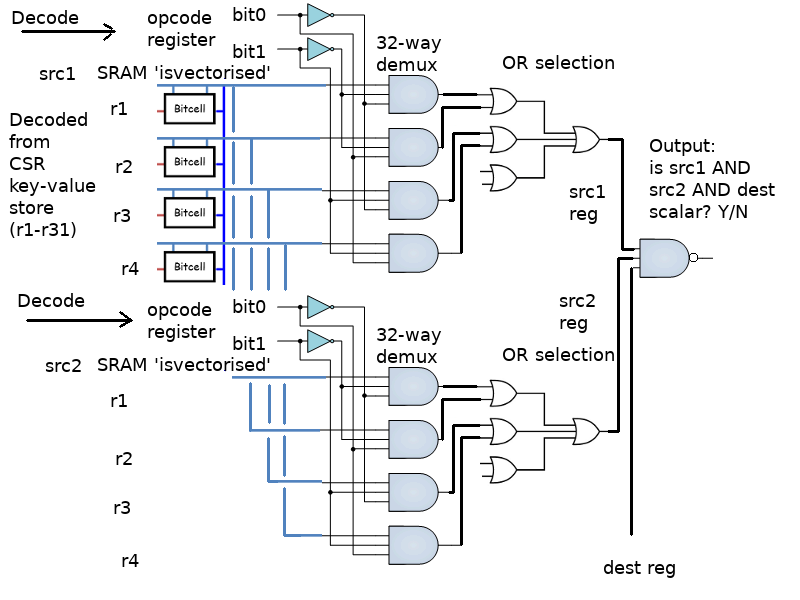
\includegraphics[height=2.5in]{scalardetect.png}\\
  {\bf \red Detect when all registers are scalar for a given op}
 \end{center}
}


\frame{\frametitle{TODO (break into separate slides)}

 \begin{itemize}
   \item    Then explain why this proposal is a good way to \\
   abstract parallelism\\
   (hopefully also explaining how \\
   a good compiler can make clever use of this increase parallelism\\
   Then explain how this can be implemented (at instruction\\
   issue time???) with\\
   implementation options, and what these "cost".\\
   Finally give examples that show simple usage that compares\\   
   C code\\
   RVIC\\
   RVV\\
   RVICXsimplev
  \end{itemize}
}


\frame{\frametitle{Summary}

 \begin{itemize}
   \item Designed for flexibility (graded levels of complexity)\vspace{6pt}
   \item Huge range of implementor freedom\vspace{6pt}
   \item Fits RISC-V ethos: achieve more with less\vspace{6pt}
   \item Reduces SIMD ISA proliferation by 3-4 orders of magnitude \\
	     (without SIMD downsides or sacrificing speed trade-off)\vspace{6pt}
   \item Covers 98\% of RVV, allows RVV to fit "on top"\vspace{6pt}
   \item Not designed for supercomputing (that's RVV), designed for
         in between: DSPs, RV32E, Embedded 3D GPUs etc.\vspace{6pt}
   \item Not specifically designed for Vectorisation: designed to\\
	     reduce code size (increase efficiency, just
		 like Compressed)\vspace{6pt}
  \end{itemize}
}


\frame{\frametitle{slide}

 \begin{itemize}
   \item \vspace{10pt}
  \end{itemize}
  Considerations:\vspace{10pt}
  \begin{itemize}
   \item \vspace{10pt}
  \end{itemize}
}


\frame{
  \begin{center}
    {\Huge \red The end\vspace{20pt}\\
			    Thank you}
  \end{center}
}


\end{document}
